\renewcommand{\theequation}{\theenumi}
\begin{enumerate}[label=\thesection.\arabic*.,ref=\thesection.\theenumi]
\numberwithin{equation}{enumi}

\item Let $\vec{O}$ be the centre , r be the radius and $\vec{A}=\myvec{2\\-2}$ and $\vec{B}=\myvec{3\\4}$ be the points lying on the circle.
\newline
Any point on the circle is equidistant from its centre
\begin{align}
\implies \norm{\vec{A}-\vec{O}} = \norm{\vec{B}-\vec{O}} = r
\\
\implies \norm{\vec{A}-\vec{O}}^2 - \norm{\vec{B}-\vec{O}}^2  = 0
\\
\implies \brak{\vec{A}-\vec{O}}^T\brak{\vec{A}-\vec{O}} 
\\
- \brak{\vec{B}-\vec{O}}^T\brak{\vec{B}-\vec{O}} = 0
\\
\implies \brak{\vec{A}-\vec{B}}^T\vec{O} =   \frac{\norm{\vec{A}}^2- \norm{\vec{B}}^2}{2}
\label{eq:points_circle1}
\end{align}
Also centre O lies on the line
\begin{align}
\myvec{1&1} \vec{X} = 2
\\
\myvec{1&1} \vec{O} = 2
\label{eq:line_circle1}
\end{align}

\eqref{eq:points_circle1} and \eqref{eq:line_circle1}, can be combined to form the matrix equation
\begin{align}
\vec{N}\vec{O} &= \vec{c}
\\
\implies \vec{O} &= \vec{N}^{-1} \vec{c}
\label{eq:finding_centre1}
\end{align}
%
where 
%
\begin{align}
\vec{N} &= \myvec{\brak{\vec{A}-\vec{B}}^{T} \\ \myvec{1&1}}
\\
\vec{c} &= \myvec{\frac{\norm{\vec{A}}^2- \norm{\vec{B}}^2}{2} \\ 2}
\end{align}
radius r of the circle is given as
\begin{align}
r &= \norm{\vec{A}-\vec{O}}
\label{eq:finding_radius1}
\end{align}
Therefore the equation of the circle is 
\begin{align}
\norm{\vec{X}-\vec{O}} &=r
\end{align}
Where O and r are derived using equations \ref{eq:finding_centre1} and \ref{eq:finding_radius1}

The following code calculates centre and radius and plots figure \ref{fig:circle1}
\begin{lstlisting}
codes/circle1/circle1.py.py
\end{lstlisting}
\begin{figure}[!ht]
\centering
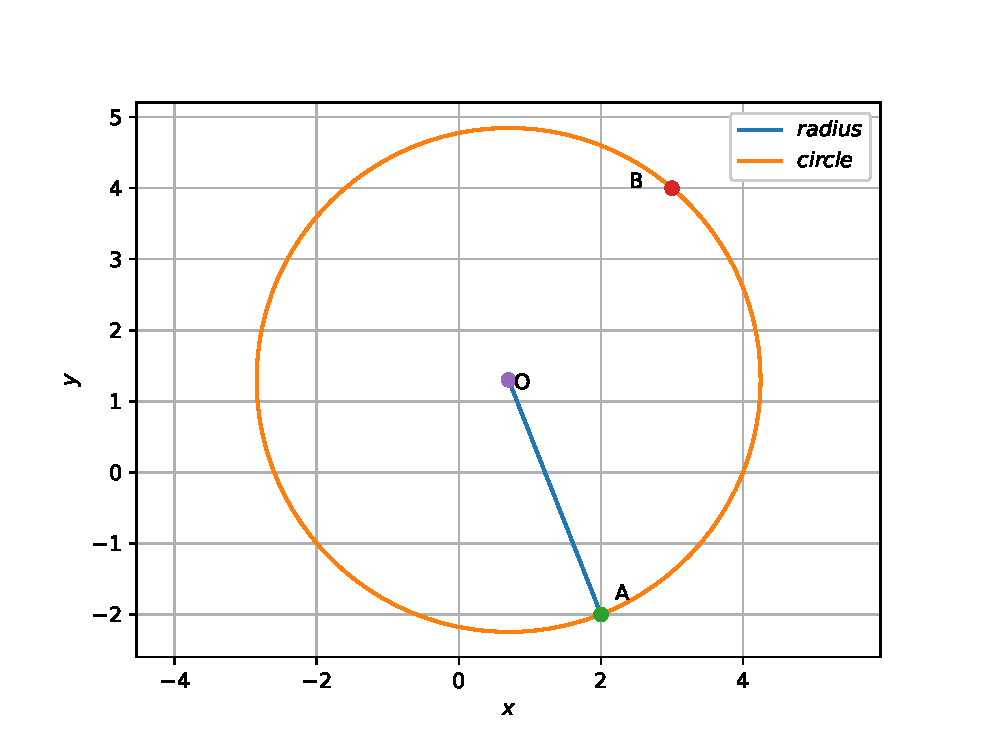
\includegraphics[width=\columnwidth]{./codes/circle1/pyfigs/circle1.eps}
\caption{Circle with centre at $\vec{O}$ and radius r}
\label{fig:circle1}
\end{figure}

\end{enumerate}
